\documentclass[8pt]{beamer}
%\usepackage[T1]{fontenc}% pour la sortie
\usepackage[utf8]{inputenc}
\usepackage{amsmath}
\usepackage{mathrsfs}
\usepackage{amssymb}
\usepackage{xcolor}
\usepackage{fancyhdr}
\usepackage{color}
\usepackage{bm}
\usepackage{cases}
\usepackage{comment}
\usepackage{tabto}

\usepackage{pict2e}
\usepackage{pgfplots}

\usepackage{graphicx}
\usepackage{kbordermatrix} 

\usepackage{tikz}
\usetikzlibrary{tikzmark}
\usetikzlibrary {graphs,shapes.geometric}
 
\usepackage{multimedia}
\usepackage{sidecap}

\usepackage{hanging}

\usepackage[natbib=true,style=authoryear,backend=bibtex,useprefix=true]{biblatex}
\addbibresource{bib.bib}

\setbeamertemplate{footnote}{%
  \hangpara{0.8em}{1}%
   \makebox[-0.4em][l]{\scriptsize\insertfootnotemark}\scriptsize\insertfootnotetext\par%
}

\newcommand*{\Scale}[2][4]{\scalebox{#1}{$\displaystyle{#2}$}}%
\newcommand{\ml}[1]{\textcolor{blue}{[\emph{ML} -- #1]}}


\usefonttheme[onlymath]{serif} %% Pour écrire les maths comme dans les documents latex classiques
\setbeamertemplate{navigation symbols}{} %% Pour enlever les symboles de navigation en bas à droite, peu utiles
  
% \usetheme{Warsaw}
\usetheme{Frankfurt}

\setbeamercolor{structure}{fg =blue!70}

\definecolor{mygreen}{rgb}{0, 0.6, 0}

\renewcommand{\kbldelim}{(}% Left delimiter
\renewcommand{\kbrdelim}{)}% Right delimiter

%%% Définition de l'en-tête de page
\setbeamercolor{headcolor1}{fg=white,bg=blue!70}
\setbeamercolor{headcolor2}{fg=white,bg=red!75}


\makeatletter

\def\insertnavigation#1{%
  \vbox{{%
    \usebeamerfont{section in head/foot}\usebeamercolor[fg]{section in head/foot}%
    \beamer@xpos=0\relax%
    \beamer@ypos=1\relax%
    \hbox to #1{\hskip.3cm\setbox\beamer@sectionbox=\hbox{\kern1sp}%
      \ht\beamer@sectionbox=1.875ex%
      \dp\beamer@sectionbox=0.75ex%
        \hskip.3cm%
        \global\beamer@section@min@dim\z@
        \dohead%
        \beamer@section@set@min@width
      \box\beamer@sectionbox\hfill\hskip.3cm}%
}}}%  
\setbeamertemplate{caption}[numbered]
\setbeamertemplate{headline}
{%
  \begin{beamercolorbox}[ht=2.25ex,dp=3.75ex]{headcolor1}
    \hskip-4ex\insertnavigation{\paperwidth}
  \end{beamercolorbox}%
}



%% Définition du pied de page
\setbeamercolor{footcolor}{fg=white,bg=blue!70}

\setbeamertemplate{footline}{
\leavevmode%
\hbox{\hspace*{-0.08cm}
\begin{beamercolorbox}[wd=.2\paperwidth,ht=2.7ex,dp=1ex,center]{footcolor}%
	\insertshortauthor
\end{beamercolorbox}%
\begin{beamercolorbox}[wd=.6\paperwidth,ht=2.7ex,dp=1ex,center]{footcolor}%
	\insertshorttitle
\end{beamercolorbox}%
\begin{beamercolorbox}[wd=.1\paperwidth,ht=2.7ex,dp=1ex,center]{footcolor}%
	\vspace{-0.07cm}
\includegraphics[width=0.3cm]{figures/bacteria.png}\hspace*{2em}
\includegraphics[width=0.3cm]{figures/bacteria_2.png}
%	\insertframenumber{} / \inserttotalframenumber\hspace*{2ex}
\end{beamercolorbox}}%
\begin{beamercolorbox}[wd=.1\paperwidth,ht=2.7ex,dp=1ex,right]{footcolor}%
	\insertframenumber{} / \inserttotalframenumber\hspace*{2ex}
\end{beamercolorbox}%
\vskip0pt%
}

\makeatother
\author[Maxime LECOMTE]{Présenté par Maxime LECOMTE \vspace{-0.5cm}}
\title[Hybrid approach for explainable metabolic modelling of microbial ecosystems']{Approche hybride de modélisation explicable du métabolisme des écosystèmes microbiens}
\subtitle{Hybrid approach for explainable metabolic modelling of microbial ecosystems'}
\date{\today}

\usetikzlibrary{shapes,backgrounds}


\begin{document}

\begin{frame}

\maketitle
\small
{\centering\itshape Membres du jury\par}
Président: SIMON Laurent\par\medskip

\begin{tabular}[t]{@{}l@{\hspace{3pt}}p{.35\textwidth}@{}}
Rapportrices: & BAROUKH Caroline\\
& COCAIGN-BOUSQUET Muriel
\end{tabular}%
\newline

\begin{tabular}[t]{@{}l@{\hspace{3pt}}p{.32\textwidth}@{}}
Examinateurs: 
& COTTRET Ludovic \\
& LAROCHE Béatrice \\
& MARKOV Gabriel \vfill
\end{tabular}%
\footnotesize
\begin{tabular}[t]{@{}l@{\hspace{4pt}}p{.4\textwidth}@{}}
Co-direction: & David SHERMAN et Hélène FALENTIN \\
Encadrement: & Clémence FRIOUX
\end{tabular}%


\includegraphics[height=0.55cm]{figures/logos/logo_EDMI.png}
\hfill

\includegraphics[height=0.55cm]{figures/logos/Logo-INRAE_Transparent.png}
\hfill

\includegraphics[height=0.55cm]{figures/logos/logo_inria.png}
\hfill

\includegraphics[height=0.55cm]{figures/logos/logo_LaBRI.png}

\end{frame}



%%%%%%%%%%%%%%%%%%%%%%%%%%%%%%%%%%%%%%%%%%%%%%%%%%%%%%%%%%%%%%%%%%%%%%%%%%%%%%%%%%%
\section{Motivation}

\begin{frame}
\frametitle{Why the study of microorganisms is relevant ?}
\centering
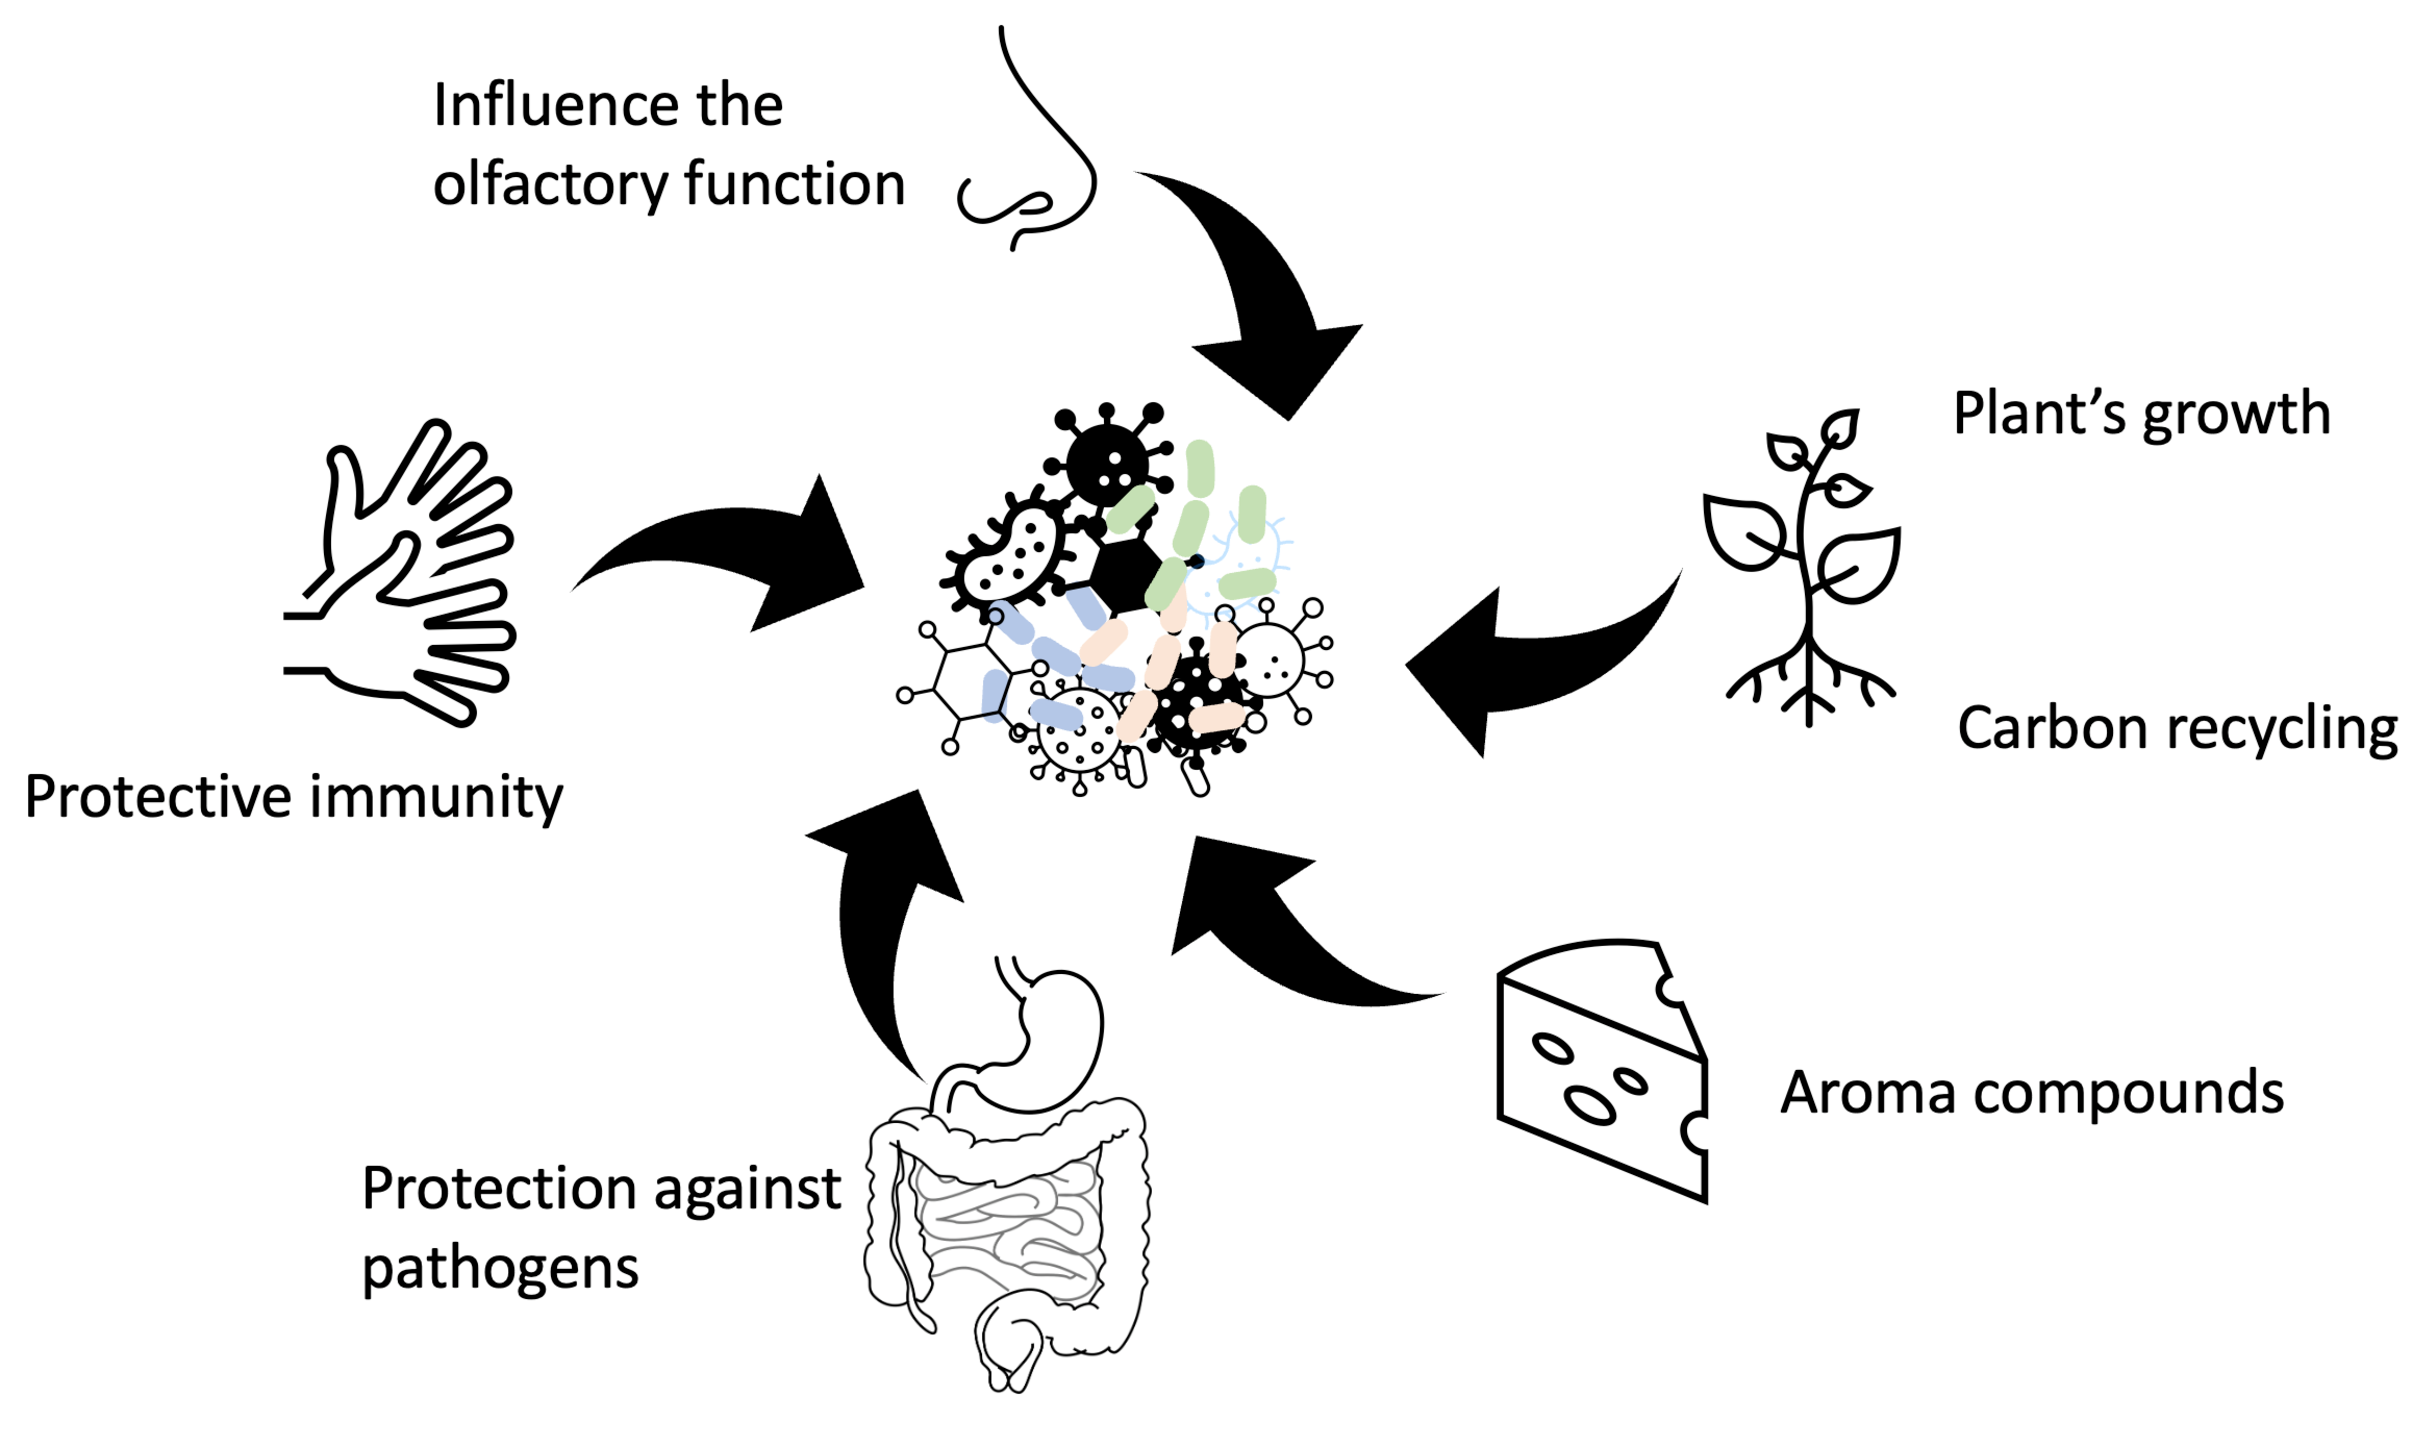
\includegraphics[width=\textwidth]{figures/bacterial-env.pdf}

\begin{block}{}
\begin{itemize}
\item High diversity of microorganisms
\item Microorganisms roles specific to the environment \tiny\citep{10.1093/chemse/bjh067,BELKAID2014121,Zhang2015,Hoorman2011,McSweeney2000}
\end{itemize}
\end{block}
\end{frame}


\begin{frame}
\frametitle{What underlying mechanisms are responsible of the observed activity ?}
\only<1>{
\framesubtitle{Metabolism}
\begin{minipage}{0.4\textwidth}
\begin{figure}
	\centering
	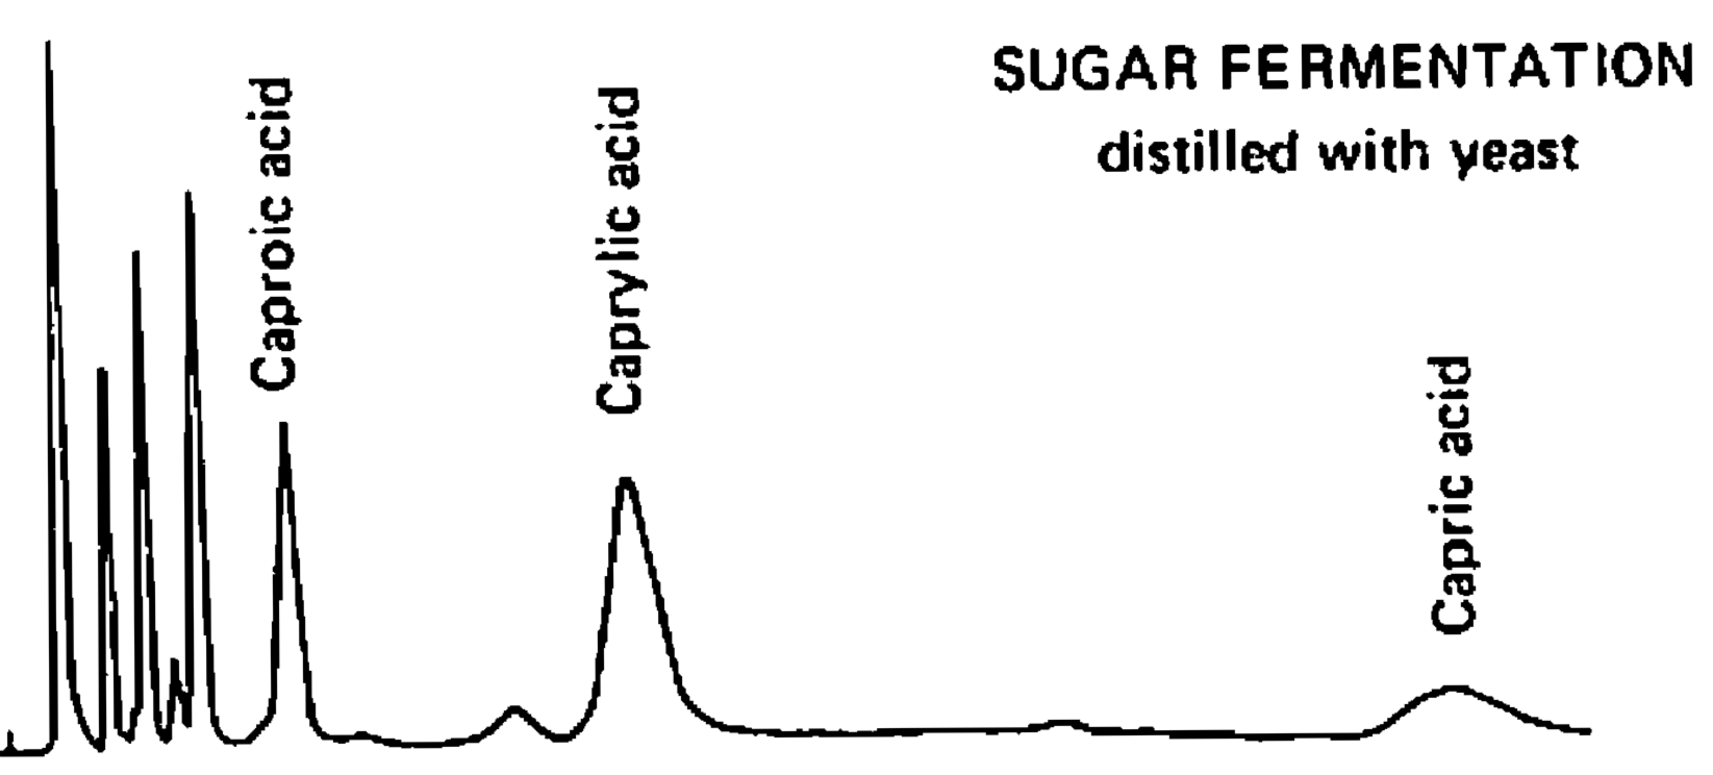
\includegraphics[width=0.9\textwidth]{figures/aroma-cpd-rum}
    \caption{Gas chromatograms of the major aroma compounds isolated from rum  \tiny (from \cite{Suomalainen1978})}
\end{figure}
\end{minipage}%
}

\only<2>{
\framesubtitle{Metabolism}
\begin{minipage}{0.4\textwidth}
\begin{figure}
	\centering
	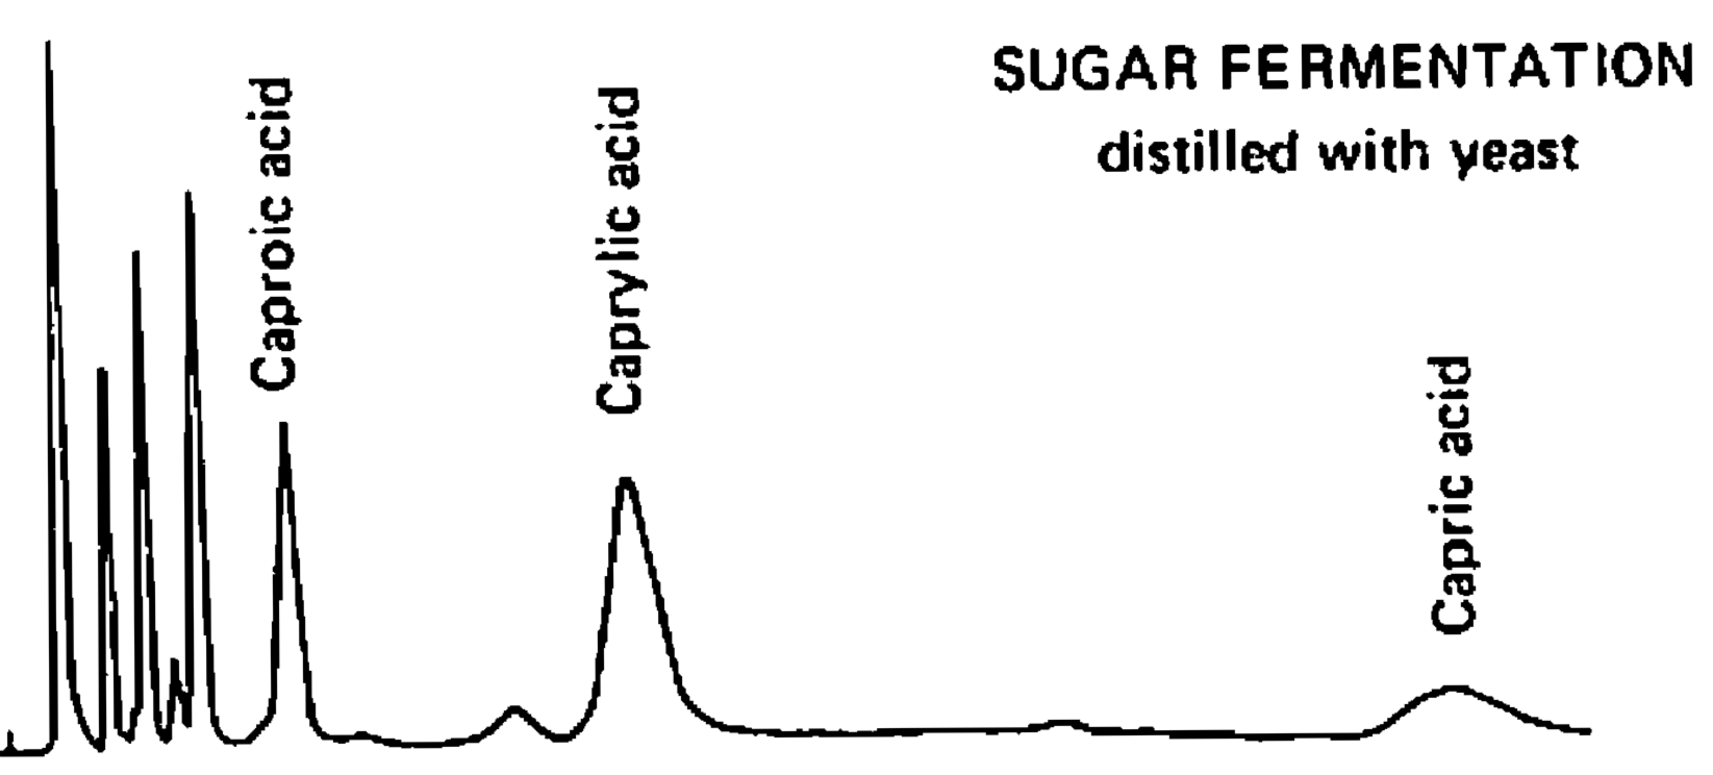
\includegraphics[width=0.9\textwidth]{figures/aroma-cpd-rum}
    \caption{Gas chromatograms of the major aroma compounds isolated from rum  \tiny (from \cite{Suomalainen1978})}
\end{figure}0
\vspace{-0.7cm}
\begin{exampleblock}{What is metabolism ?}
Set of all biochemical reactions occurring in the cell of an organism that permit the production of energy and metabolic goods. \tiny \citep{Nava2023}
\end{exampleblock}
\end{minipage}
}

\only<3>{
\frametitle{What underlying mechanisms are responsible of the observed activity ?}
\framesubtitle{Metabolism and Bacterial interactions}
\begin{minipage}{0.4\textwidth}
\begin{figure}
	\centering
	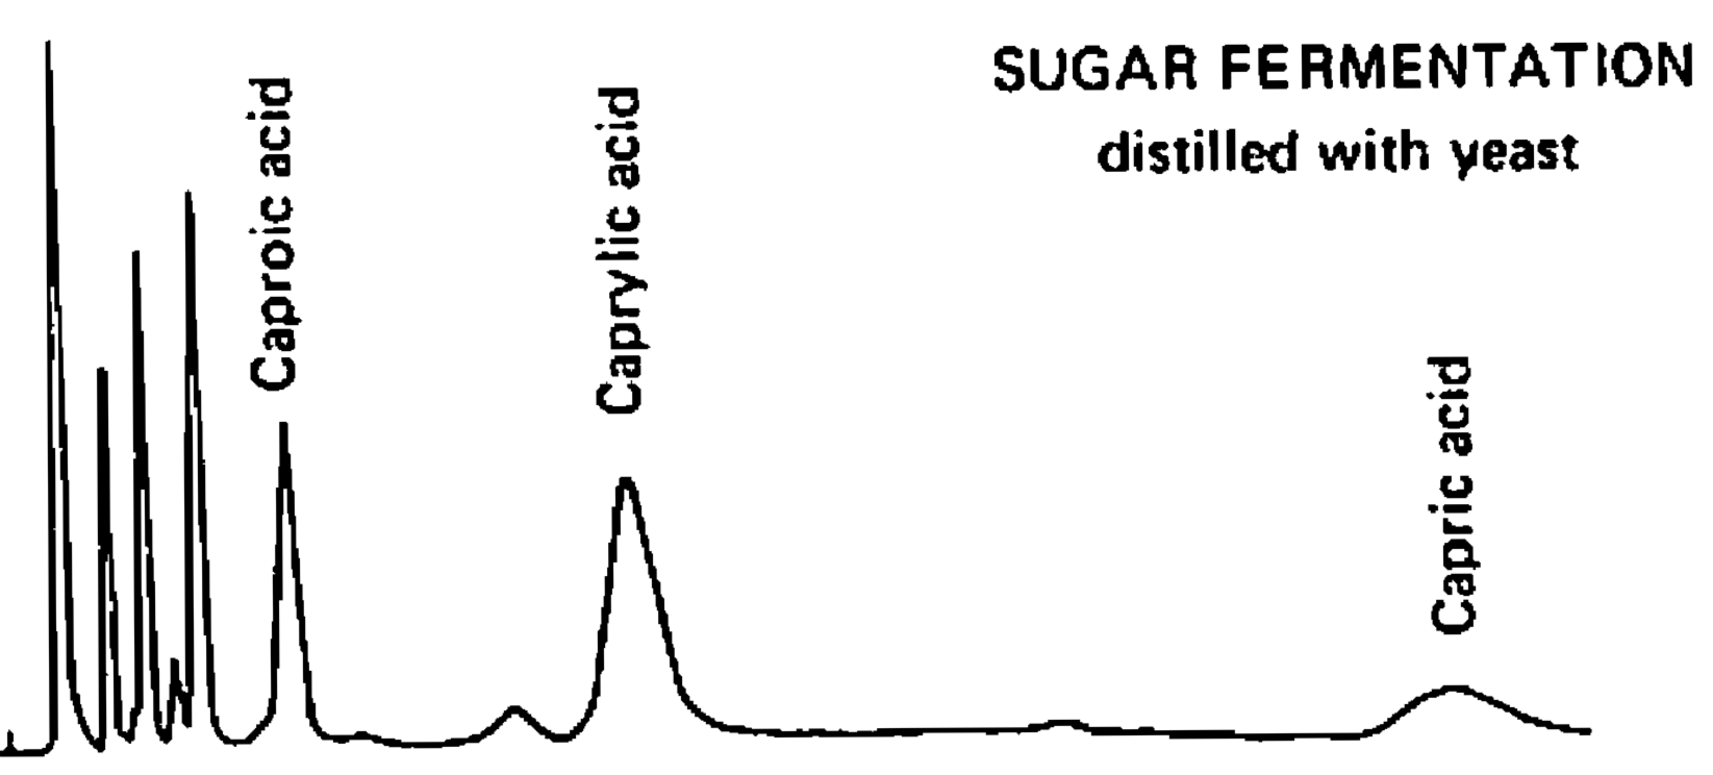
\includegraphics[width=0.9\textwidth]{figures/aroma-cpd-rum}
    \caption{Gas chromatograms of the major aroma compounds isolated from rum  \tiny (from \cite{Suomalainen1978})}
\end{figure}
\vspace{-0.7cm}
\begin{exampleblock}{What is metabolism ?}
Set of all biochemical reactions occurring in the cell of an organism that permit the production of energy and metabolic goods. \tiny \citep{Nava2023}
\end{exampleblock}
a fatty acyl-CoA + ethanol $\rightarrow$ ethyl palmitate + coA
\begin{itemize}
\item Metabolism of an organism explain observable phenotype
\end{itemize}
\end{minipage}%
}

\only<4>{
\frametitle{What underlying mechanisms are responsible of the observed activity ?}
\framesubtitle{Metabolism and Bacterial interactions}
\begin{minipage}{0.4\textwidth}
\begin{figure}
	\centering
	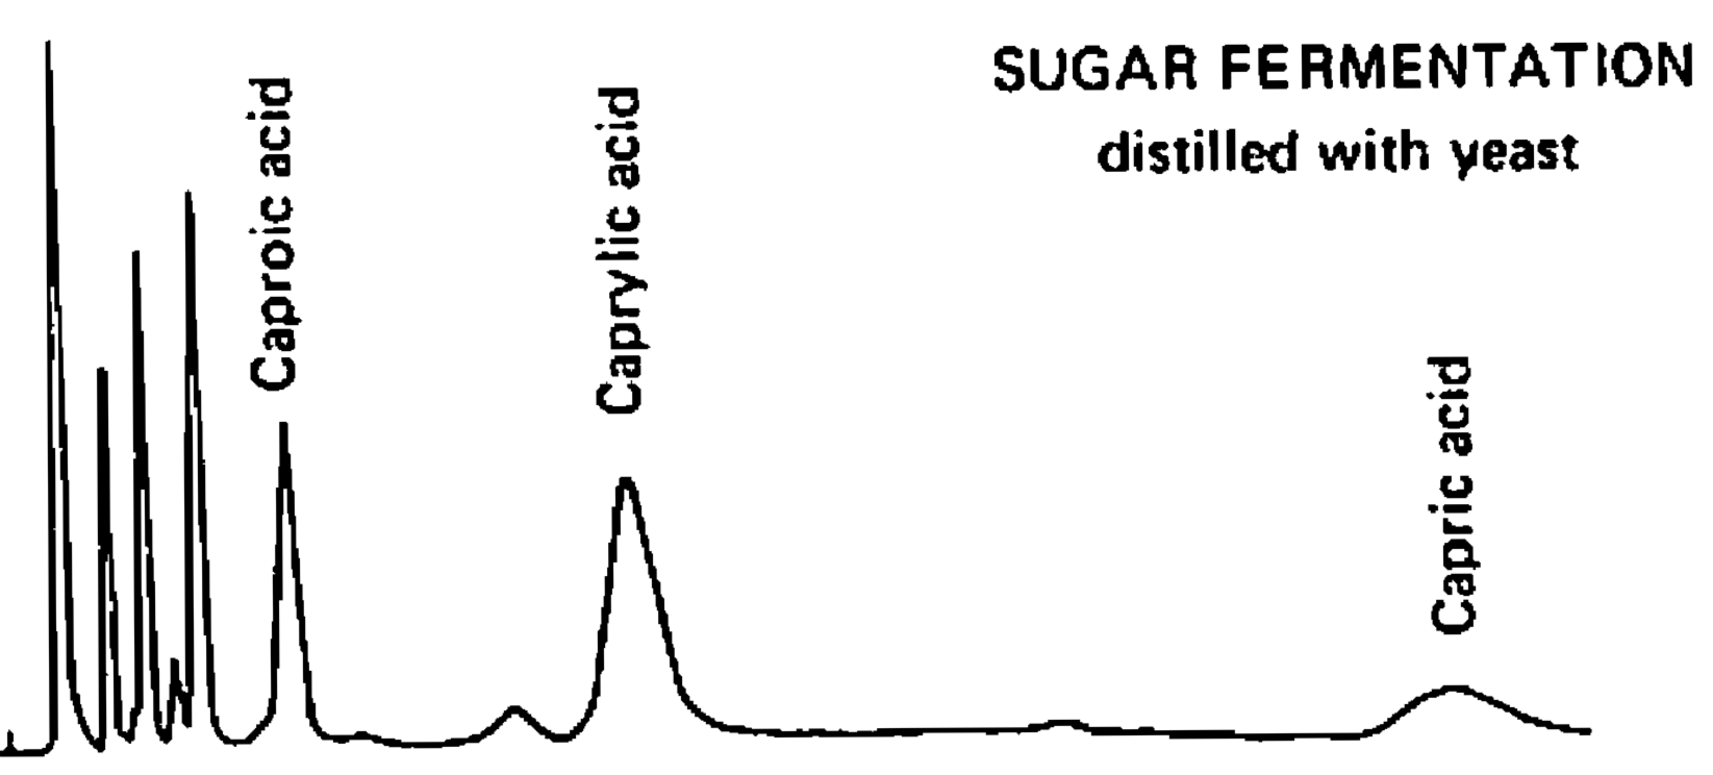
\includegraphics[width=0.9\textwidth]{figures/aroma-cpd-rum}
    \caption{Gas chromatograms of the major aroma compounds isolated from rum  \tiny (from \cite{Suomalainen1978})}
\end{figure}
\vspace{-0.7cm}
\begin{exampleblock}{What is metabolism ?}
Set of all biochemical reactions occurring in the cell of an organism that permit the production of energy and metabolic goods. \tiny \citep{Nava2023}
\end{exampleblock}
a fatty acyl-CoA + ethanol $\rightarrow$ ethyl palmitate + coA
\begin{itemize}
\item Metabolism of an organism explain observable phenotype
\end{itemize}
\end{minipage}%
\hspace{0.1\textwidth}%
\begin{minipage}{0.5\textwidth}
\begin{figure}
	\centering
	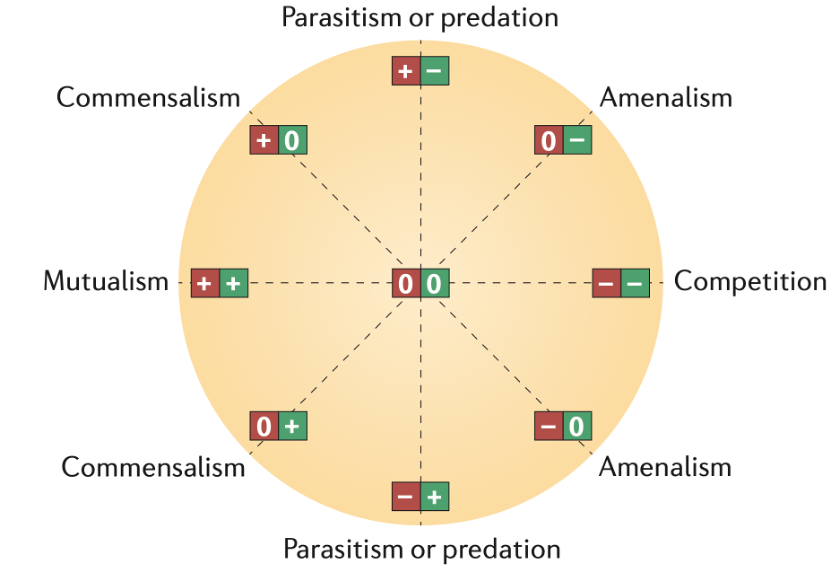
\includegraphics[width=\textwidth]{figures/interaction.png}
    \caption{List of different types of bacterial interactions \tiny \citep{Faust2012} }
\end{figure}
\begin{itemize}
\item Bacterial interaction can affect positively / negatively other organisms
\end{itemize}
\end{minipage}
}

\only<5>{
\frametitle{What underlying mechanisms are responsible of the observed activity ?}
\framesubtitle{Metabolism and Bacterial interactions}
\begin{minipage}{0.4\textwidth}
\begin{figure}
	\centering
	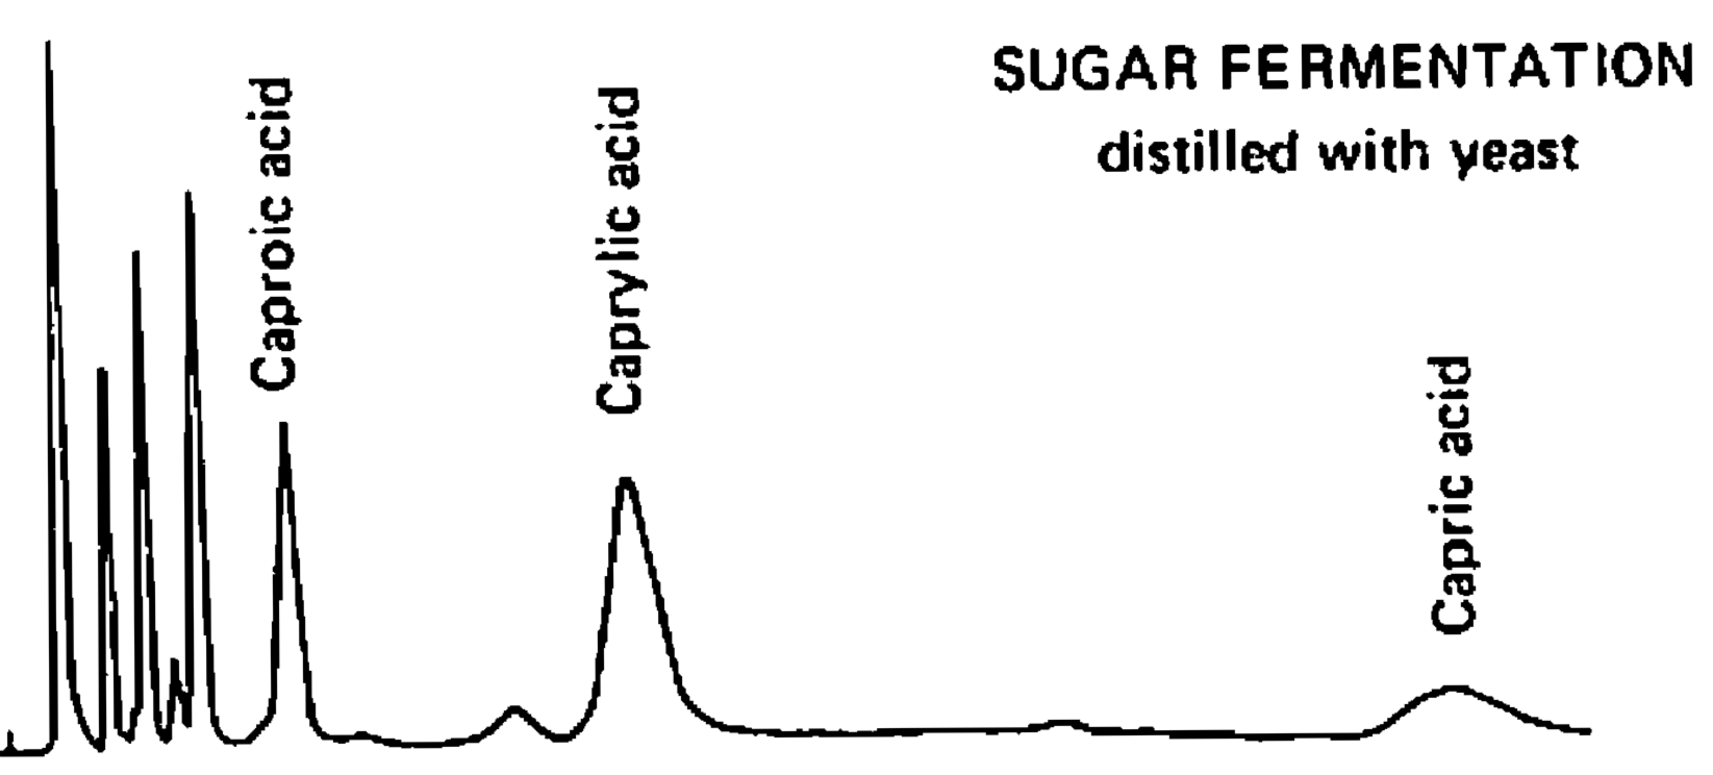
\includegraphics[width=0.9\textwidth]{figures/aroma-cpd-rum}
    \caption{Gas chromatograms of the major aroma compounds isolated from rum  \tiny (from \cite{Suomalainen1978})}
\end{figure}
\vspace{-0.7cm}
\begin{exampleblock}{What is metabolism ?}
Set of all biochemical reactions occurring in the cell of an organism that permit the production of energy and metabolic goods. \tiny \citep{Nava2023}
\end{exampleblock}
a fatty acyl-CoA + ethanol $\rightarrow$ ethyl palmitate + coA
\begin{itemize}
\item Metabolism of an organism explain observable phenotype
\end{itemize}
\end{minipage}%
\hspace{0.1\textwidth}%
\begin{minipage}{0.5\textwidth}
\begin{figure}
	\centering
	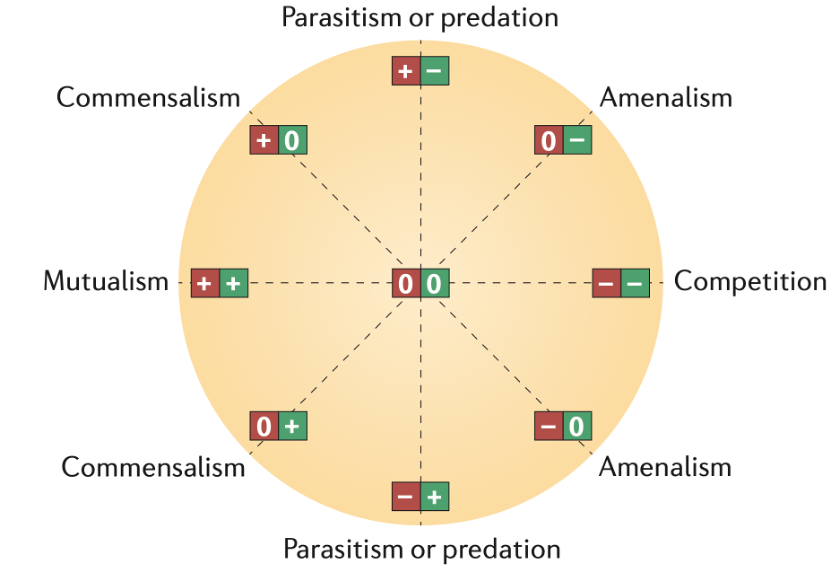
\includegraphics[width=\textwidth]{figures/interaction.png}
    \caption{List of different types of bacterial interactions \tiny \citep{Faust2012} }
\end{figure}
\begin{itemize}
\item Bacterial interaction can affect positively / negatively other organisms
\end{itemize}
\end{minipage}
\begin{block}{}

Bacterial interactions can modulate metabolic goods

\end{block}}
\end{frame}

\begin{frame}
\frametitle{How can we study this impact through metabolism? }
\framesubtitle{Genome-scale metabolic network (GEMs) reconstruction}
\begin{figure}
\centering
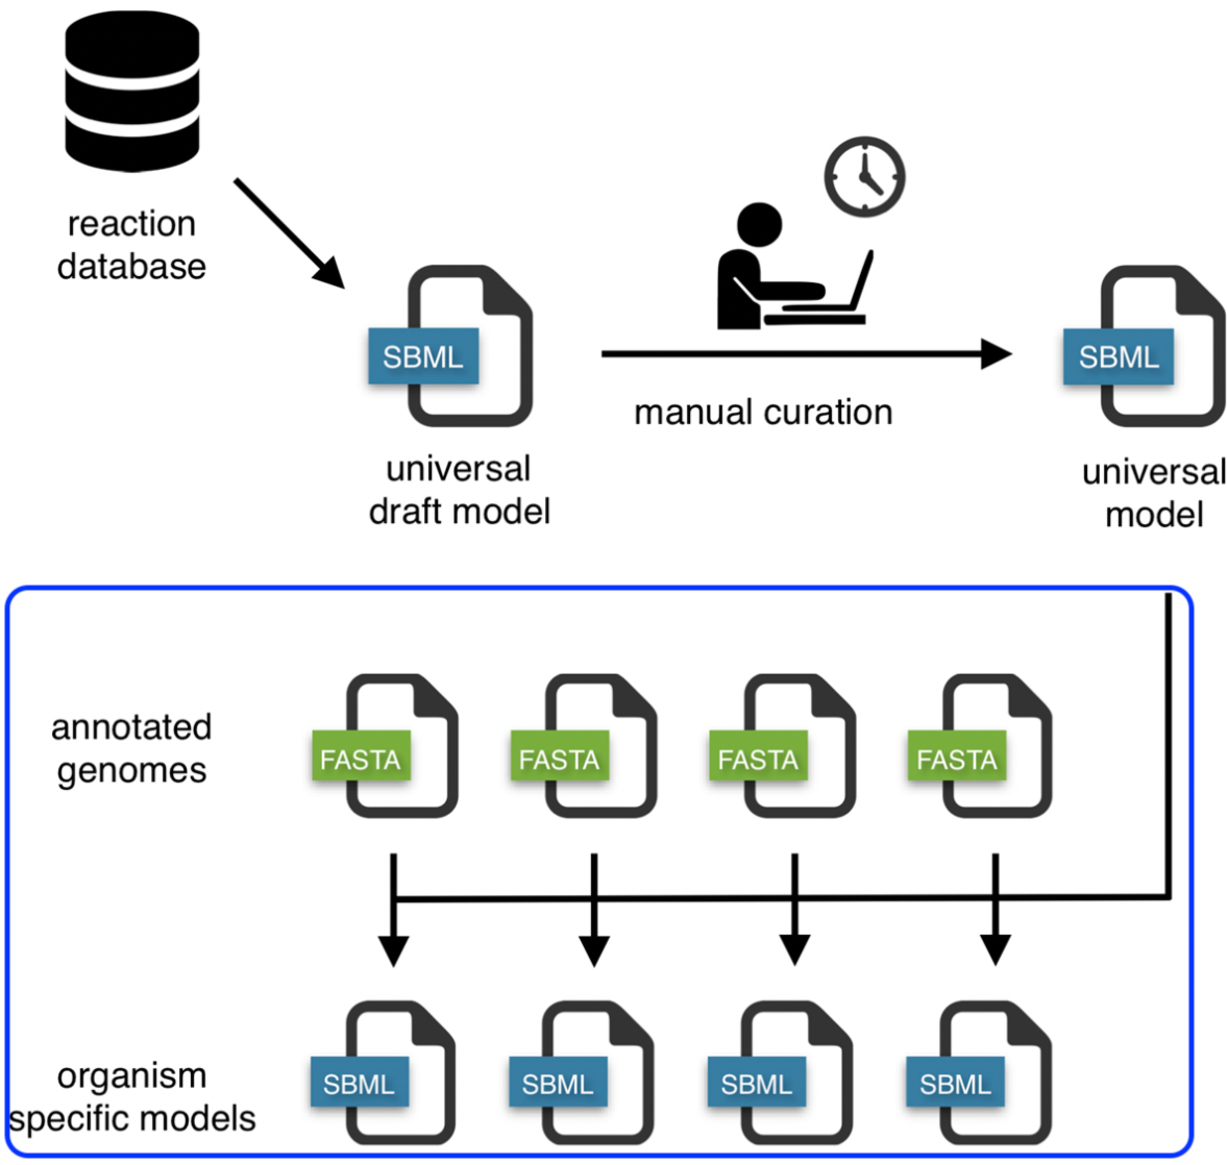
\includegraphics[width=0.55\textwidth]{figures/top-down}
\caption{Top down genome-scale metabolic network reconstruction approach \tiny (modified from \cite{Machado2018})}
\end{figure}
\begin{itemize}
\item For bacteria: average of 1500 reactions, 1000 genes, 800 metabolites
\item Informatic can help to resolve combinatorial problem
\end{itemize}
\end{frame}

%
%\begin{frame}{Quels sont les apports biologiques et informatiques d'étudier les bactéries}
%\centering
%\begin{tikzpicture}
%	\begin{scope} [fill opacity = .4]
%    \draw[fill=green, draw = black] (-1.5,1) circle (3);
%    \draw[fill=blue, draw = black] (1.5,1) circle (3);
%
%        \node at (2.5,2) {\LARGE\textbf{Simulate}};
%    \node at (0,2) {\LARGE\textbf{Explain}};
%    \node at (2.5,1) {\LARGE\textbf{Prediction}};
%    \node at (0,1) {\LARGE\textbf{Generate}};
%    \node at (0,0.5) {\LARGE\textbf{hypothesis}};
%    \node at (-3,2) {\LARGE\textbf{Identifivation}};
%    \node at (-3,1) {\LARGE\textbf{Improvement}};
%%\draw[help lines](-5,5) grid (5,-6); %%%   This line can draw the grid lines to help guide you. I use these when I'm writing the code and then delete this line when I publish th
%    \end{scope}
%
%        \node at (-3.5,4) {\LARGE\textbf{Biology}};
%    \node at (3.5,4) {\LARGE\textbf{Informatic}};
%
%\end{tikzpicture}
%
%\begin{block}{}
%\begin{itemize}
%\item L'informatique semble nécessaire pour affiner l'étude des bactéries
%\end{itemize}
%\end{block}
%\end{frame}

\begin{frame}
\frametitle{How can we study this impact through metabolism? }
\framesubtitle{Systems biology}
\begin{exampleblock}{System biology}
Associate an organism to a system and study the all system \tiny \citep{Kitano2002}
\end{exampleblock}
\begin{minipage}{0.8\textwidth}
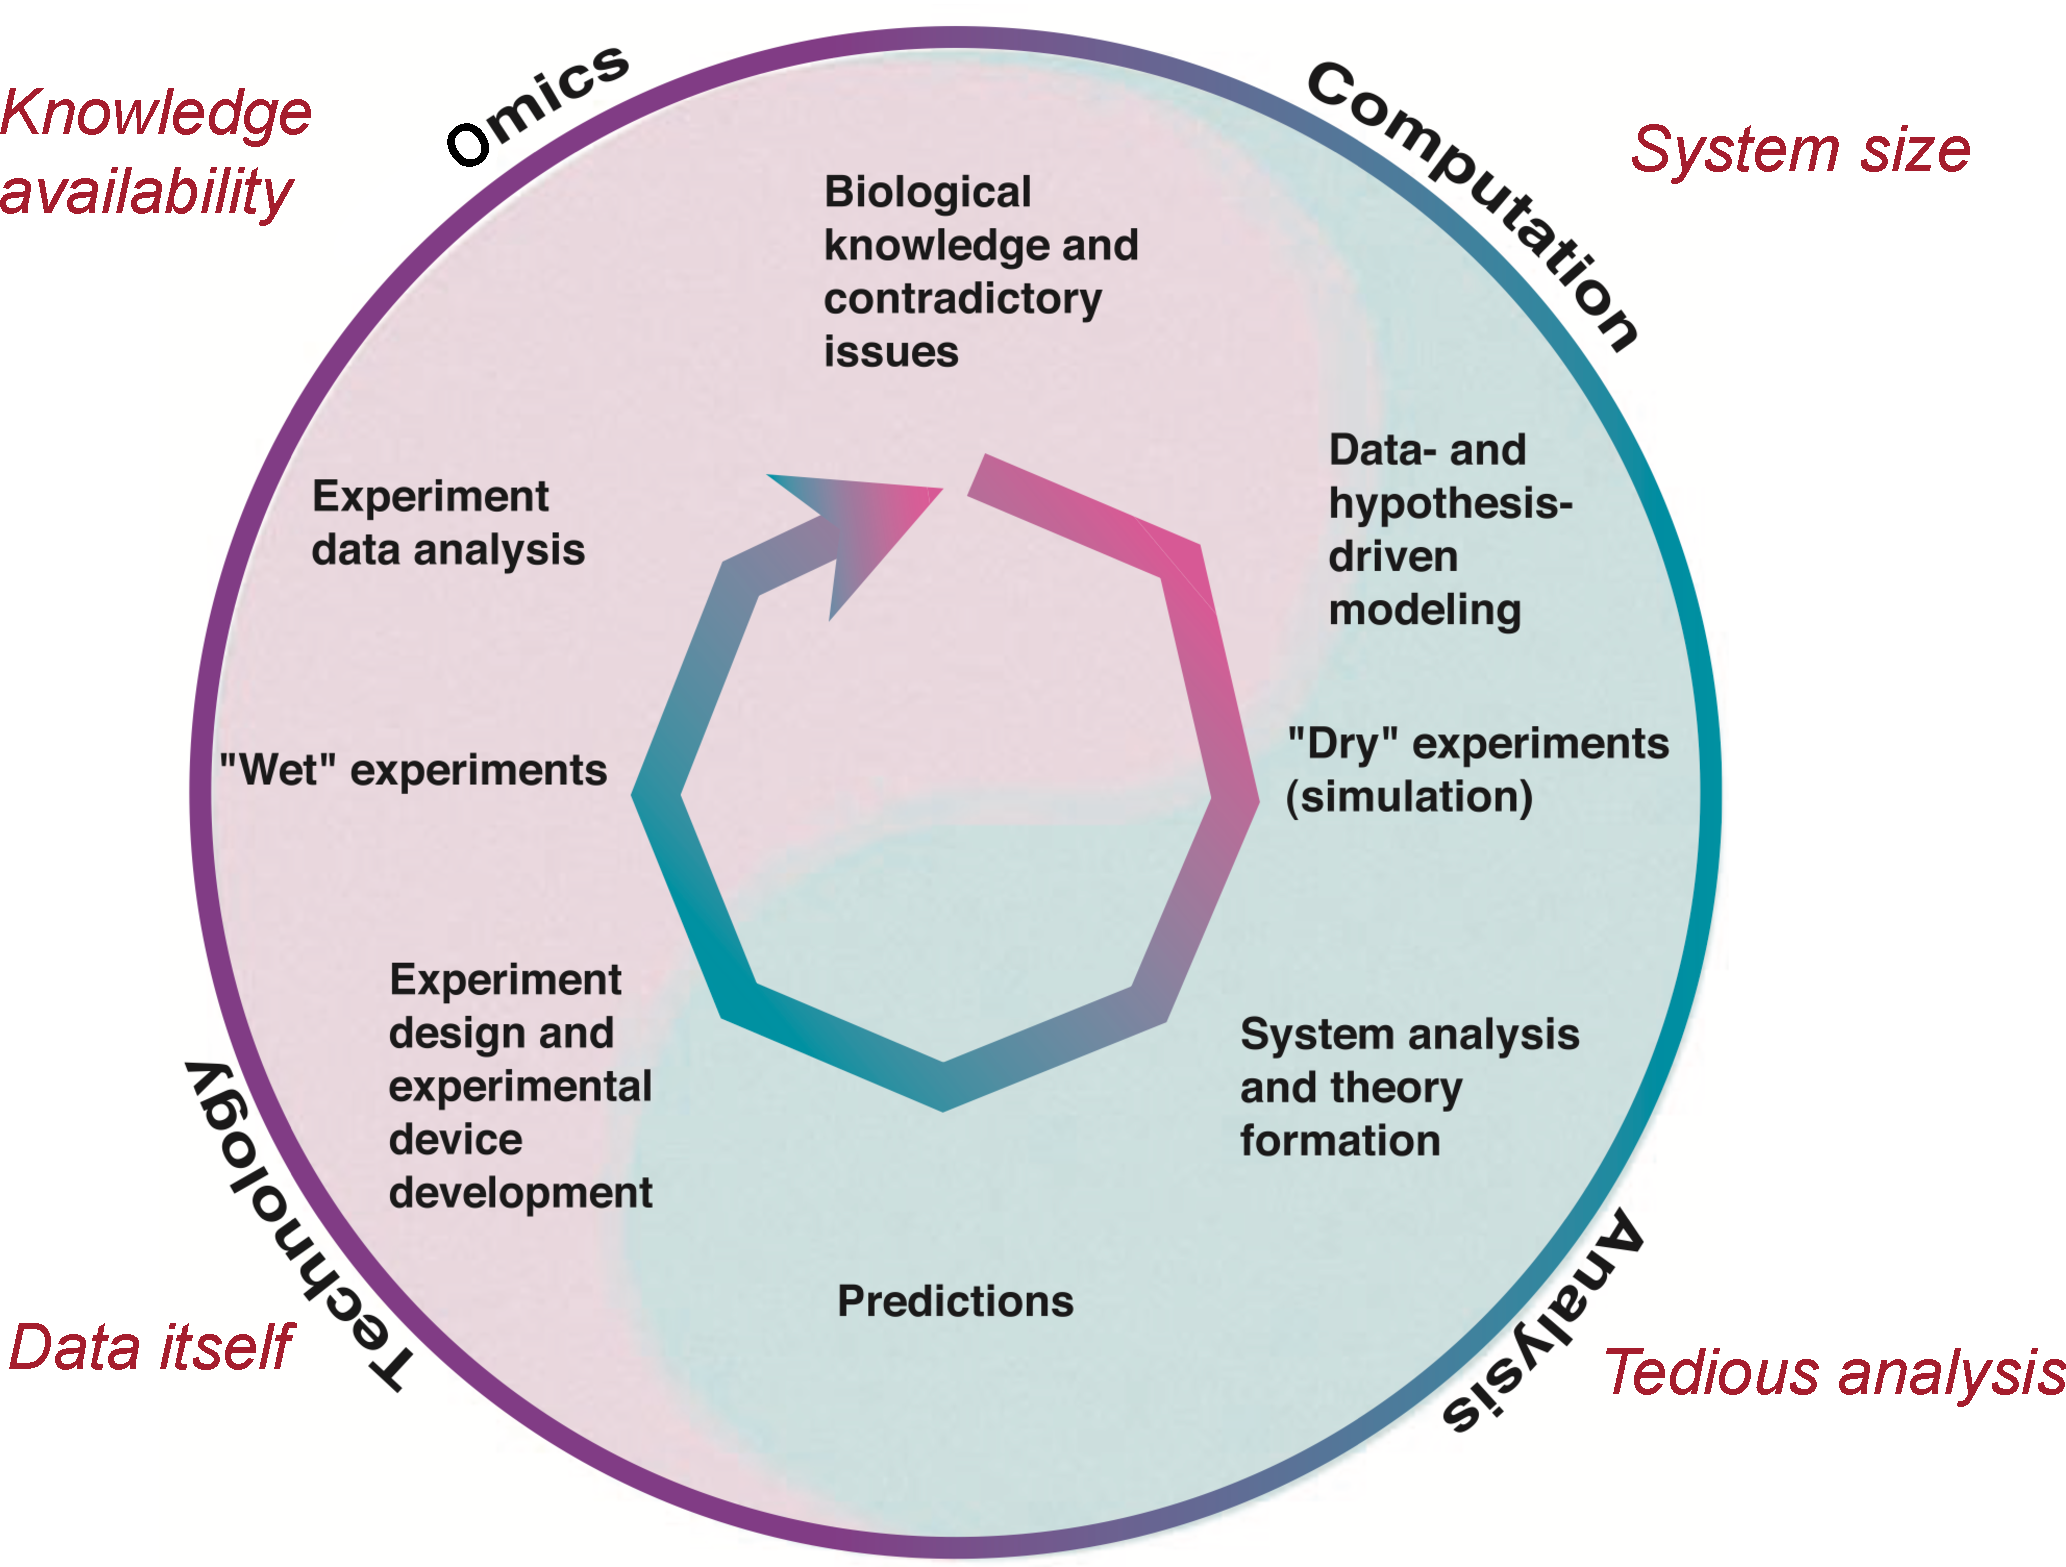
\includegraphics[width=\textwidth]{figures/systeme-biology.pdf}
\end{minipage}%
\begin{minipage}{0.2\textwidth}
\begin{figure}
\caption{System biology modified from \cite{Kitano2002}}
\end{figure}
\end{minipage}
\vspace{-0.2cm}
\begin{block}{}
\begin{itemize}
\item System biology combines biology and informatic analysis for studying bacterial behavior
\end{itemize}
\end{block}
\end{frame}


\section{Background}
\begin{frame}
\frametitle{How the computational phase is concretely achieve ?}
\framesubtitle{Metabolic network representation}
\only<1>{
$r_1 : $2 pyr $\rightarrow$ 1 acetoL + 1 $\text{CO}_2$ \\
$r_2 : $1 acetoL  $\rightarrow$ 1 diac  + 1 $\text{CO}_2$ \\ 
$r_3 : $1 acetoL  $\rightarrow$ 1 acetoin + 1 $\text{CO}_2$ \\
$r_4 : $1 diac $\rightarrow$ 1 acetoin \\
$r_5 : $1 acetoin  $\rightarrow$1 butanediol \\

}

\only<2>{

$r_1 : $2 pyr $\rightarrow$ 1 acetoL + 1 $\text{CO}_2$ \\
$r_2 : $1 acetoL  $\rightarrow$ 1 diac  + 1 $\text{CO}_2$ \\ 
$r_3 : $1 acetoL  $\rightarrow$ 1 acetoin + 1 $\text{CO}_2$ \\
$r_4 : $1 diac $\rightarrow$ 1 acetoin \\
$r_5 : $1 acetoin  $\rightarrow$1 butanediol \\


\begin{minipage}{0.5\textwidth}
\textbf{Stoichiometry matrix}


\[
  \kbordermatrix{
     & r_1  & r_2 & r_3 & r_4 & r_5 \\
    \text{pyr}                                           & -2 & 0 & 0 & 0 & 0 \\
    \text{acetoL}                      & 1 & -1 & -1 & 0 & 0  \\
    \text{diac}                      & 0 & 1 & 0 & -1 & 0  \\
    \text{CO}_2         & 1 & 1 & 1 & 0 & 0    \\
    \text{acetoin}         & 0 & 0 & 1 & 1 & -1   \\
    \text{butanediol}         & 0 & 0 & 0 & 0 & 1  \\
        }
\]


\end{minipage}%
\begin{minipage}{0.5\textwidth}


\end{minipage}
}

\only<3>{

$r_1 : $2 pyr $\rightarrow$ 1 acetoL + 1 $\text{CO}_2$ \\
$r_2 : $1 acetoL  $\rightarrow$ 1 diac  + 1 $\text{CO}_2$ \\ 
$r_3 : $1 acetoL  $\rightarrow$ 1 acetoin + 1 $\text{CO}_2$ \\
$r_4 : $1 diac $\rightarrow$ 1 acetoin \\
$r_5 : $1 acetoin  $\rightarrow$1 butanediol \\


\begin{minipage}{0.5\textwidth}
\textbf{Stoichiometry matrix}
\[
  \kbordermatrix{
     & r_1  & r_2 & r_3 & r_4 & r_5 \\
    \text{pyr}                                           & -2 & 0 & 0 & 0 & 0 \\
    \text{acetoL}                      & 1 & -1 & -1 & 0 & 0  \\
    \text{diac}                      & 0 & 1 & 0 & -1 & 0  \\
    \text{CO}_2         & 1 & 1 & 1 & 0 & 0    \\
    \text{acetoin}         & 0 & 0 & 1 & 1 & -1   \\
    \text{butanediol}         & 0 & 0 & 0 & 0 & 1  \\
        }
\]
\end{minipage}%
\begin{minipage}{0.5\textwidth}
\textbf{bipartite graph}

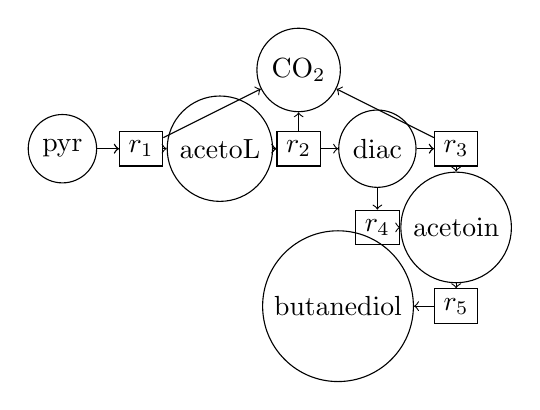
\begin{tikzpicture}
\node (x) [circle, draw] at (0,0)   {pyr};
  \node (a) [circle, draw] at (2,0)   {acetoL};
    \node (b) [circle, draw] at (4,0)   {diac};
      \node (c) [circle, draw] at (3,1)   {$ \text{CO}_2 $};
        \node (d) [circle, draw] at (5,-1)   {acetoin};
          \node (e) [circle, draw] at (3.5,-2)   {butanediol};
          
  \node (f) [rectangle, draw] at (1,0) {$r_1$};
  	\node (g) [rectangle, draw] at (3,0)  {$r_2$};
  	  \node (h) [rectangle, draw] at (5,0)   {$r_3$};
  		\node (i) [rectangle, draw] at (4,-1)   {$r_4$};
  		  \node (j) [rectangle, draw] at (5,-2)   {$r_5$};

  \graph { (x) -> (f) -> (a) };
   \graph { (x) -> (f) -> (c) };
   \graph { (a) -> (g) -> (c) };
    \graph { (a) -> (g) -> (b) };
	\graph { (b) -> (h) -> (c) };      
	 \graph { (b) -> (h) -> (d) };            
	 	 \graph { (b) -> (i) -> (d) };       
	 	 	 	 \graph { (d) -> (j) -> (e) };                 
	 
\end{tikzpicture}

\end{minipage}

\begin{block}{}
\textbf{Stoichiometry matrix} is commonly used for quantitative analysis instead of \textbf{graph}, more focused on topology analysis
\end{block}


}


\end{frame}


\begin{frame}
\only<1>{
\frametitle{How the computational phase is concretely achieve ?}
\framesubtitle{Build a metabolic model}
\begin{exampleblock}{Metabolic model}
From a GEM, a model metabolic has the capacity to simulate and to predict on the metabolic content
\end{exampleblock}
}

\only<2>{
\frametitle{How the computational phase is concretely achieve ?}
\framesubtitle{Build a metabolic model}
\begin{exampleblock}{Metabolic model}
From a GEM, a model metabolic has the capacity to simulate and to predict on the metabolic content
\end{exampleblock}
\begin{minipage}{0.5\textwidth}
\textbf{Constraint-based approaches}
\[
\frac{dx}{dt} = S . v = 0
\]

\end{minipage}

}


\end{frame}

\begin{frame}{Objectifs de la thèse}

\end{frame}

\tiny
\printbibliography


\end{document}
